\chapter{Collaboration in Virtual Environments} %\chapter{Collaboration in Similar Projects}

Collaboration can be approached in different ways, depending on the task at hand. More traditional approach is with \gls{cscw} systems, it works well when the task is routine and just requires either information exchange, or an execution of a pre-defined task \cite{churchill_collaborative_1998}. For more creative and non-trivial tasks, which can be obscured by enforcing a certain workflow early-on, an approach using \gls{cve} is more appropriate.

\paragraph{}
% CVEs
One of the origins of \gls{cve}s is the field of \gls{vr}. This is mostly due to the aim  to allow users creative freedom, and reduce the learning curve by providing an intuitive interface. The task of a \gls{cve} is to facilitate communication and collaboration. They allow synchronous and asynchronous task execution, and provide the support for real-time sharing of visual artifacts \cite{churchill_collaborative_1998}.

\subparagraph{}
% Cocoverse, Greenwald
A good and concise review of the history of the \gls{cve}s can be found in \cite{greenwald_technology_2017}. The state of art in the area of CVEs was reached by one of the authors, in \cite{greenwald_cocoverse_nodate} and \cite{greenwald_investigating_2017} he presents CocoVerse - a shared immersive \gls{vr} environment for local collaboration and co-creation (Fig. \ref{fig:cocoverse}).

\begin{figure}
	\centering
	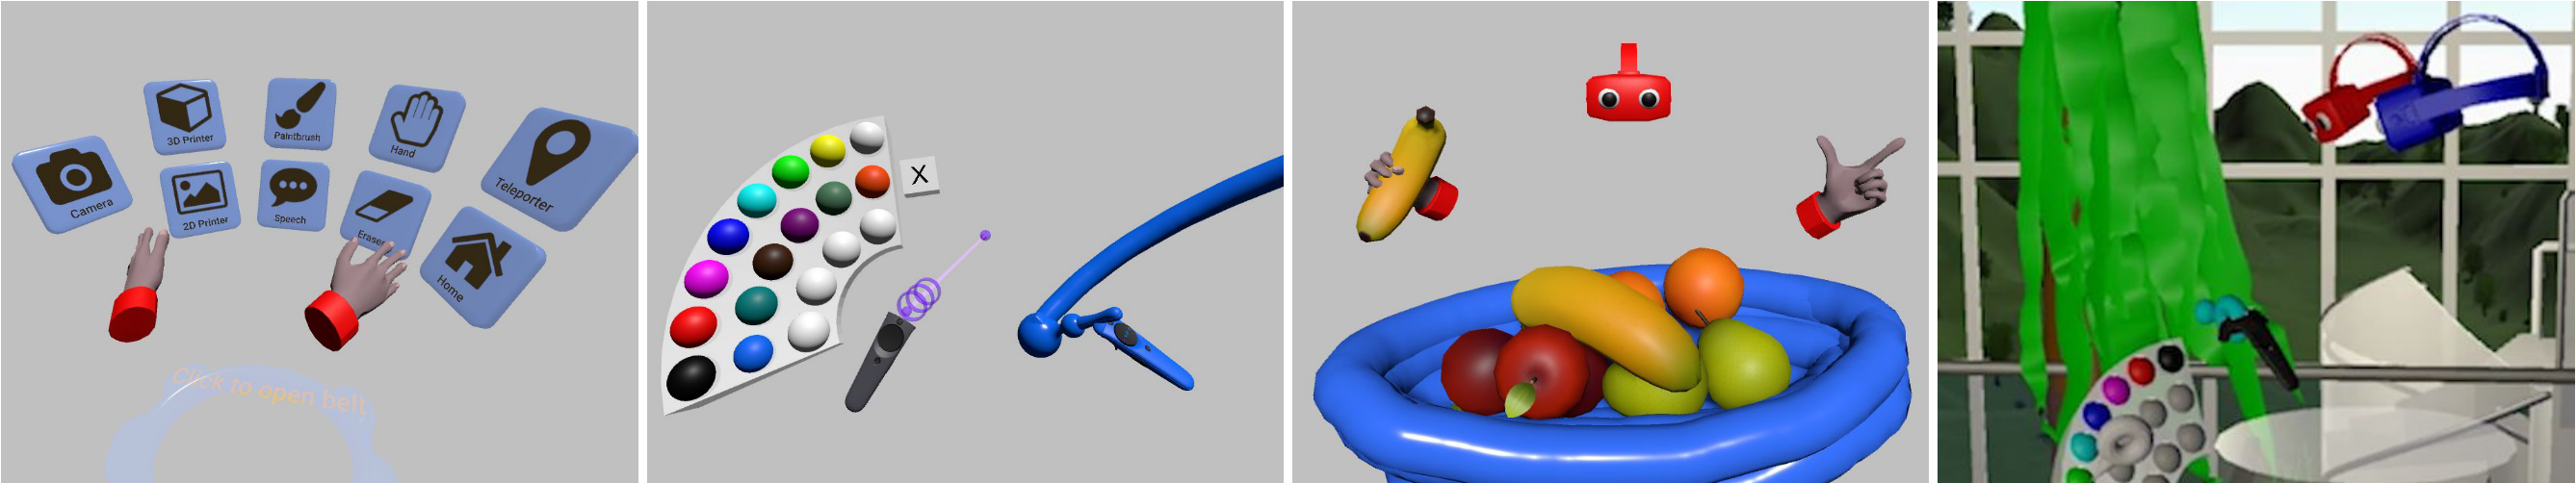
\includegraphics[width=0.7\linewidth]{figures/Cocoverse}
	\caption{CocoVerse, environment affordances and avatars (Source: \cite{greenwald_cocoverse_nodate})}
	\label{fig:cocoverse}
\end{figure}

%% What they explored, their focus and discoveries
%%% Goals
Authors' main research direction is communication, collaboration, and learning in \gls{vr}. As the field of immersive \gls{vr} is relatively young, one of the main goals of those projects was to explore the feasibility and utility of such setup, and pilot methodologies for studying behavior in this setting (\cite{greenwald_investigating_2017}). The utility was analyzed by comparing different activities in the 2D viewing mode (via a monitor) and as the immersive 3D experience.

%%% Setup/system
The system is a room-scale shared immersive \gls{vr} experience, which allows users to synchronously manipulate the environment with a set of hand-based tools (create 3D drawings, communicate via rough hand gestures, etc.). CocoVerse also lets the users know where others are looking, by providing them with minimalistic avatars that convey the gaze direction. Users require either a \gls{hmd} and a pair of 6 \gls{dof} controllers to use the system in the immersive mode, or simply a PC to participate in the 2D mode.

%%% Focus and the results
Authors report the overall success and promise of such setups as an engine for learning and creativity. They further review, how the sense of social presence is influenced by the complexity of avatars and high movement realism. \cite{greenwald_investigating_2017} proposes guidelines for deciding on the level of sophistication of the embodiment based on the type of experience that is being digitalized.

\subparagraph[CSCW]{}
% Concise: what other CVE projects addressed.
Among other CVEs that were explored, \cite{lena_real-time_nodate} proposes a system, which connects two different mediums (an interactive table computer, and a CAVE-environment), and focuses on the way to develop consistent interactions across the environment. % TODO: more (e.g. Kulik)

% Conclusion: something else is needed
Generally, it seems that the focus of the modern \gls{cve} projects is more on exploring the aspects of the intentional communication and interactions, where users are always aware of each other during the collaboration task. I our case, the focus should be more on consequential communication, which arises as a result of user's actions.

% CSCWs
We will now turn to the field of \gls{cscw}, which is regarded by \cite{churchill_collaborative_1998} as the main way to approach the automation of the collaborative work, before the paradigm shift towards \gls{cve}s. \gls{cscw} applications also provide distributed access to a shared context. However, unlike \gls{cve}s, these applications provide a less malleable environment that is restricted by requirements of a certain workflow. Examples of \gls{cscw} applications include: emailing software, project management and conferencing tools, shared calendars and drawing tools, etc.

% Chalkboard, Gutwin
A notable work from the field of \gls{cscw} is the study presented in \cite{gutwin_chalk_2011}. The authors study the use of auditory cues to promote the up-to-the-moment understanding of another person’s interaction with the shared chalkboard application, or as they call it, the "Workspace Awareness" (WA) \cite{gutwin_descriptive_2002}. % TODO: I use the same quote in the Awareness chapter. Change.

%% What they explored, their focus and discoveries
%%% Goals
Two main goals of the study were to figure out "How much information can sound convey?" and the effectiveness of audio awareness in a \gls{cscw} application.

%%% Setup/system
The system is a 2D shared drawing application with one real (participant) and one simulated user (called an \textit{agent} in the \gls{cve} terminology). The participant has two tasks, primary and secondary. The primary task was to trace a given 2D shape (Fig. \ref{fig:gutwinchalk2011}), and the secondary was to keep track of what is happening in the shared workspace. When a participant and the agent drew, the system would emit a spatialized sound of chalk writing on a chalkboard (at a lower volume for the participant's actions). An additional way to monitor the shared environment, or as authors call it - a type of awareness presentation, was a minimap (what authors call a \textit{radar}), which showed the complete environment and the local chunk a participant was working in (indicated with a blue rectangle on the minimap).
% The workspace is seen in the figure
% Different awareness presentations - auditory and minimap
% Varying difficulty of the tracing shape

\begin{figure}
	\centering
	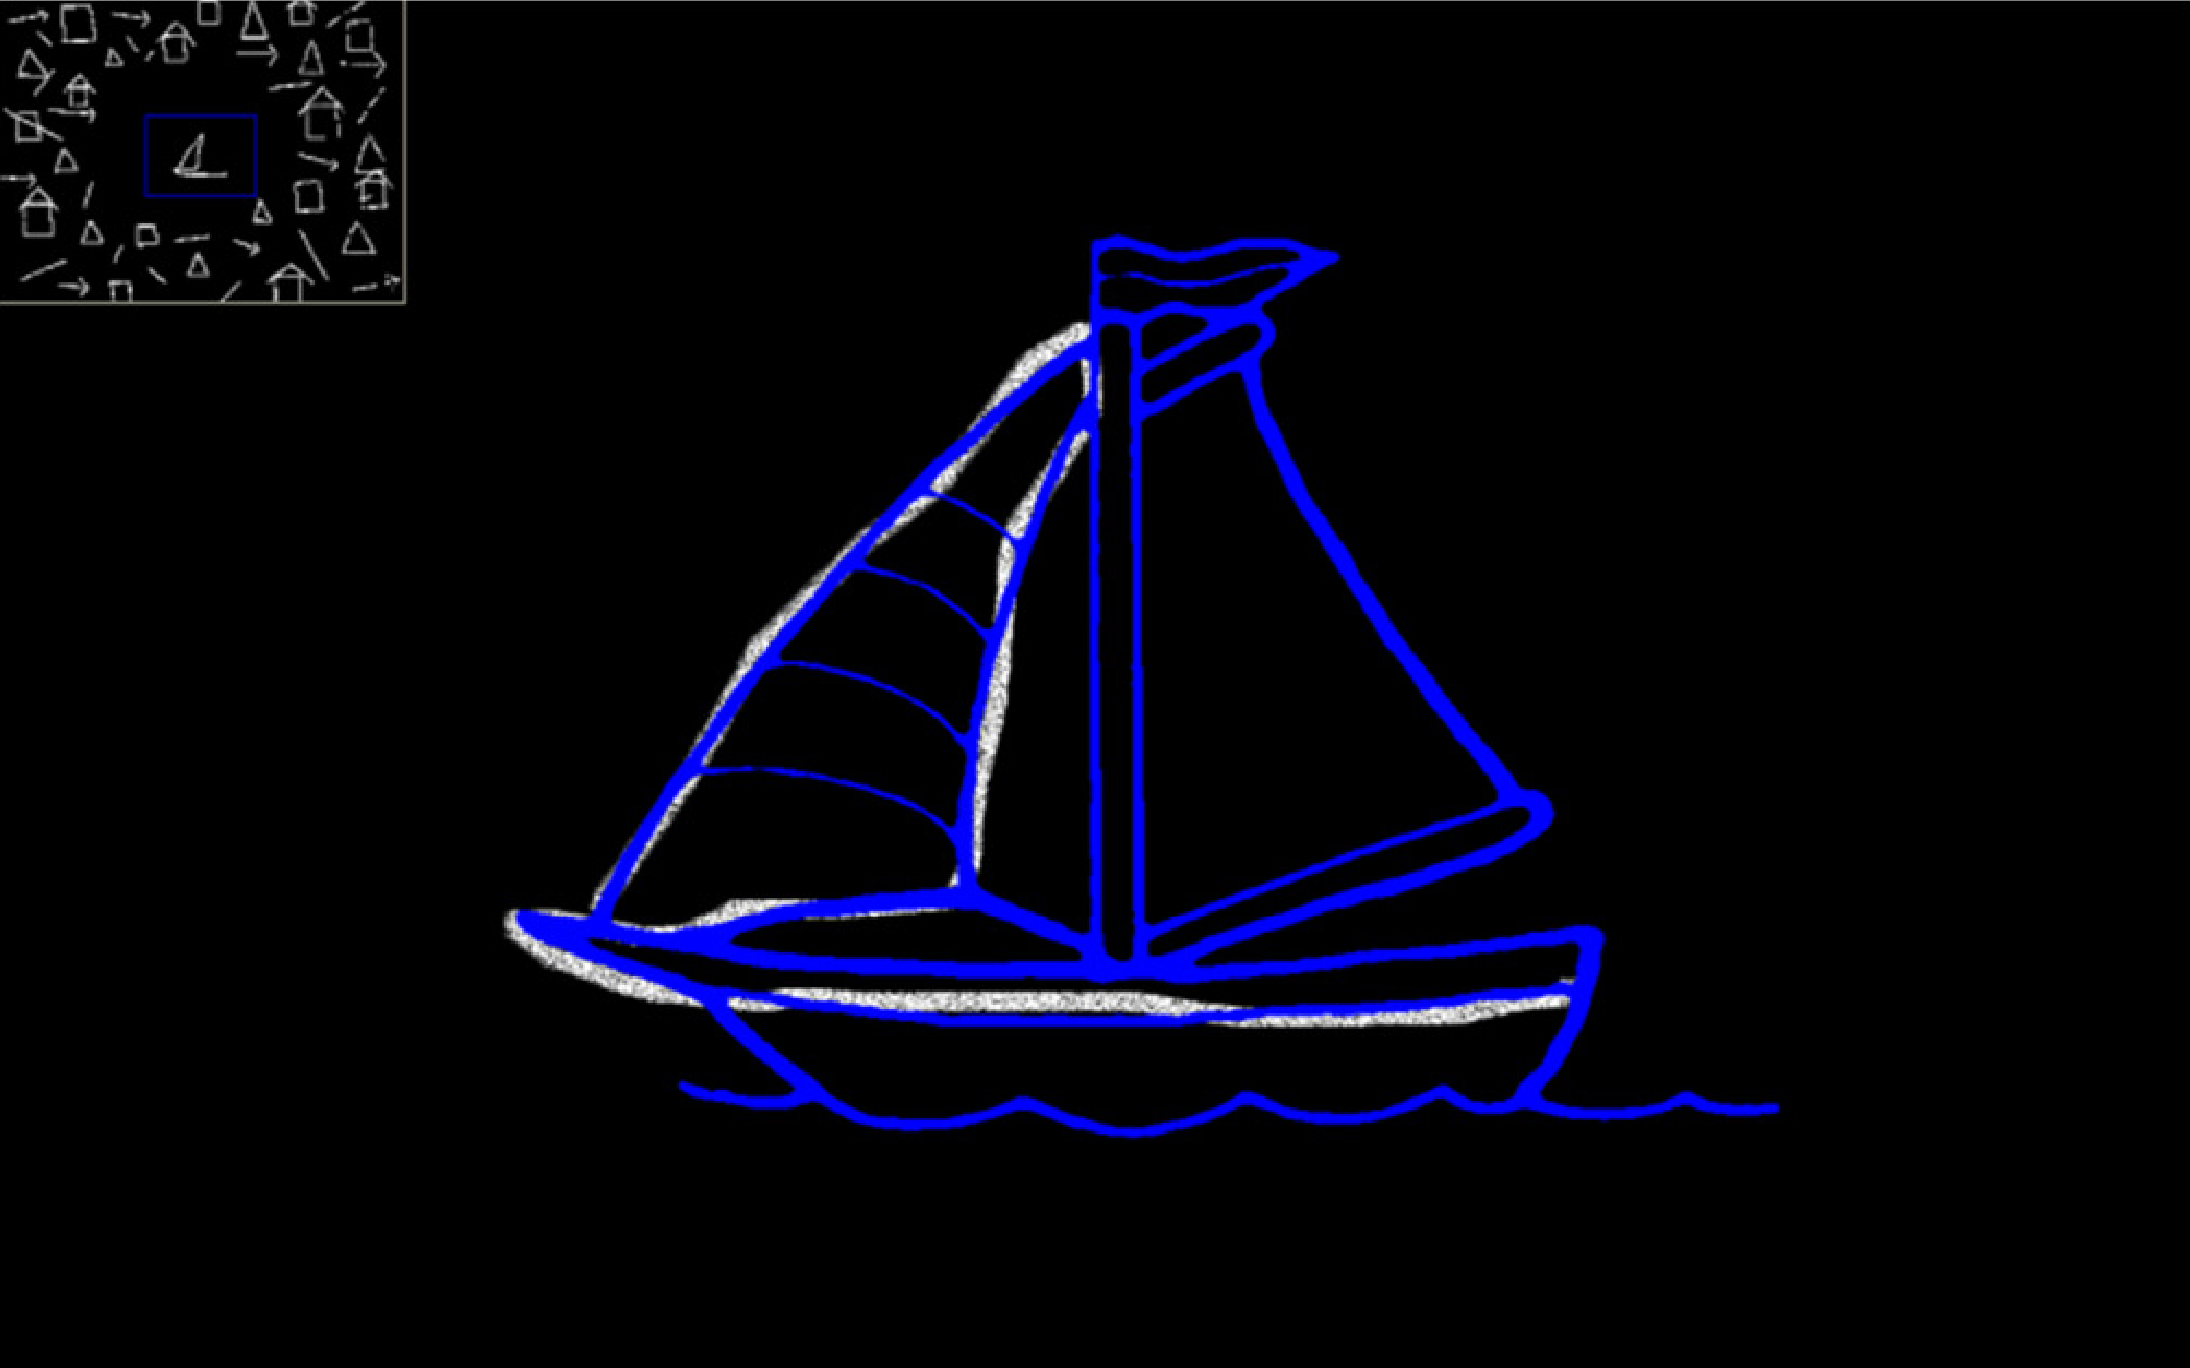
\includegraphics[width=0.7\linewidth]{figures/gutwin_chalk_2011}
	\caption{Shared chalkboard application, tracing shape and minimap (Source: \cite{gutwin_chalk_2011})}
	\label{fig:gutwinchalk2011}
\end{figure}


%%% Focus and the results
One of the characteristics of the \gls{wa} is that it is a peripheral (or a secondary) task by nature \cite{gutwin_descriptive_2002}, % TODO: I might be using the same quote in the Awareness chapter. Change.
as such, \cite{gutwin_chalk_2011} attempt to keep participant's attention on the main task by varying the difficulty of the tracing activity: the tracing shape was made to distort occasionally. Authors also study the effect of the workspace clutter, the size of the minimap, the type of auditory cues, and the awareness presentation on the \gls{wa}.

The authors report significant improvements to the group awareness in cases, where it is hard to attend to the visual displays, or the line of sight is obscured. Additionally, they provide their thoughts with regards to how and why the audio awareness helps in the collaborative scenarios, as well as the possible limitations of its application.

\paragraph[Bridge]{}
The approach used in \cite{gutwin_chalk_2011} is based on their previous work on the topic of \gls{wa} \cite{gutwin_descriptive_2002}.
Next, we are going to take a closer look at the awareness approach % TODO: did I define it?
, its history, and how it aids the design of the groupware systems. 








\begin{comment}
% Intro: Introduce what this whole chapter is about

This chapter is going describe the ?status quo of the Collaborative Virtual Environments, highlight the state of art, and the experiment on the Workspace Awareness that the practical part of this thesis took as the base.

\section{Status quo}
.. Like theory part
Define CVE, Groupware, and cooperation levels
% Talk about users and agents, cause I mention it in the experminets chapter.

\section{Related projects}
Mention some projects that are related, but won't be discussed in the detail in this work. The purpose of this subsection is to provide an overview of the current state of the groupware/collaborative software systems.
Lena
® Provides a good overview of the Collaboration and interaction in similar projects
® Focuses more on interactions …
Greenspace II
® A related work from the architectural filed
® Morally aged, Greenwald uses some findings from it
[some other works]

\section{State of art: Multi-User Framework for Collaboration and Co-Creation in Virtual Reality}
§ In this section I will discuss the work I found, which serves as the state of art for current development of Collaborative Virtual Environments (CVEs) - Multi-User Framework for Collaboration and Co-Creation in Virtual Reality (Greenwald et al. 2017).


\section{Parent/precursor/foundation work: The Effects of Dynamic Synthesized Audio on Workspace Awareness in Distributed Groupware}
§ Introduce Gutwin et al. 2011 work on The Effects of Dynamic Synthesized Audio on Workspace Awareness in Distributed Groupware (Chalk Sounds)

Goals

Setup/system
® …
® 

\begin{table}[]
	\begin{tabular}{|l|l|}
		\hline
		Number of people                                                                                  & Conceptually, multiuser                                                                                                \\ \hline
		Medium                                                                                            & PC with an interactive display for drawing                                                                             \\ \hline
		\begin{tabular}[c]{@{}l@{}}Affordances \\ (TODO: make it correspond to WA framework)\end{tabular} & \begin{tabular}[c]{@{}l@{}}Manipulation: 2D drawing, self-report\\ Communication: auditory icons, minimap\end{tabular} \\ \hline
		?Cooperation level                                                                                & Conceptually, 3.2                                                                                                      \\ \hline
		Locality                                                                                          & Shared physical space and remote collaboration                                                                         \\ \hline
	\end{tabular}
\end{table}

Focus and the results
\end{comment}
